\section{Analyse du modèle de Cox-Ross-Rubinstein}
Dans cette partie, nous nous intéresserons à la théorie du modèle de Cox-Ross-Rubinstein afin de l'implémenter dans la prochaine partie.

\subsection{Objectifs et Structure du modèle}

L'objectif du modèle \textbf{binomial} ou de \textbf{Cox-Ross-Rubinstein} est de trouver la "valeur-juste" ("fair value") d'un produit dérivé. La \textbf{fair value} est le prix auquel il n'existe aucune opportunité d'arbitrage. Ce modèle repose sur la réplication de portefeuille et la complétude de marché afin de reproduire exactement les flux futurs de l'option et de garantir l'unicité d'une probabilité risque-neutre. \\

Le modèle \textbf{Cox-Ross-Rubinstein} est un modèle de prédiction discret contrairement au modèle de \textbf{Black-Scholes} qui est continu.
Les principaux intérêts de travailler en temps discret sont la facilité de modélisation ainsi que l'implémentation algorithmique. En effet, le modèle binomial est facilement compréhensible intuitivement en représentant l'évolution des actifs sur les branches d'une arbre pondérées par les probabilités de montée et descente des prix. C'est cette modélisation qui va nous intéresser dans la suite de cette section. \\

Pour discrétiser la période de temps du call, on considère une subdivision de la période de validité de l'option en $N$ périodes de même longueur, ainsi on obtient chaque division : 
\begin{align*}
    t_n=\frac{nT}{N} ,\forall \in {0,..,N}
\end{align*}
\remarque Faire tendre $N$ vers des valeurs très grandes revient à se rapprocher d'un modèle continu. \\\\
Sur chaque subdivision, on définit deux facteurs :
\begin{center}
    \begin{itemize}
        \item[\textbf{u}] : le facteur de hausse de l'actif (up)
        \item[\textbf{d}] : le facteur de baisse de l'actif (down)
    \end{itemize}
\end{center}
Ces deux facteurs correspondent respectivement à la hausse et à la baisse du prix de l'actif. Sur un arbre, on adoptera la convention évidente qui place le facteur de hausse sur la branche la plus haute et vice-versa. \\
\\
\remarque Nous ne nous attarderons pas, dans un premier temps, sur la manière dont sont calculés ces deux facteurs.

L'algorithme se décompose donc en deux phases distinctes :
\begin{itemize}
\item \textbf{La phase de propagation (Forward) :} On part de $S_0$ pour construire l'arbre des prix du sous-jacent jusqu'à l'échéance $T$.
\item \textbf{La phase d'évaluation (Backward) :} Une fois les prix à l'échéance fixés, on calcule les \textbf{payoffs} sur les feuilles de l'arbre, puis on remonte pour déterminer la prime $S_0$
\end{itemize}
\pagebreak
\subsection{Parcours Descendant}
Représentons l'évolution du prix d'un sous-jacent ayant pour cours initial $S_0$, qui a une probabilité $p$ d'augmenter de $u$ et qui a une probabilité $1-p$ de baisser de $d$ à chaque période : 

\def\mallevel{2}
\def\ratiox{3.5} 
\def\ratioy{2.0} 

\tikzset{
   malnode/.style={draw=black, fill=white, minimum width=3.5em, circle, font=\small},
   prob/.style={midway, sloped, font=\large},
   malarrow/.style={->, >=stealth, shorten >=2pt, shorten <=2pt}
}
\begin{center}
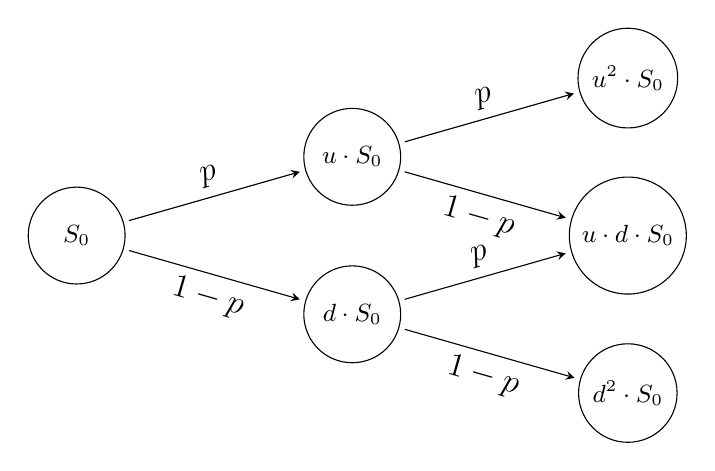
\begin{tikzpicture}
\foreach \x in {0,...,\mallevel} { 
    \foreach \y in {0,...,\x} { 
        \pgfmathsetmacro{\movey}{\y - \x/2}
        \def\nodetext{?}
        \ifnum\x=0
            \def\nodetext{$S_0$}
        \fi
        \ifnum\x=1
            \ifnum\y=1 \def\nodetext{$u \cdot S_0$} \fi
            \ifnum\y=0 \def\nodetext{$d \cdot S_0$} \fi
        \fi
        \ifnum\x=2
            \ifnum\y=2 \def\nodetext{$u^2 \cdot S_0$} \fi
            \ifnum\y=1 \def\nodetext{$u \cdot d \cdot S_0$} \fi
            \ifnum\y=0 \def\nodetext{$d^2 \cdot S_0$} \fi
        \fi
        \node[malnode] (\x-\y) at (\ratiox*\x, \ratioy*\movey) {\nodetext};

        \ifnum\x>0
            \pgfmathtruncatemacro{\prevx}{\x-1}
            \ifnum\y>0
                \pgfmathtruncatemacro{\prevyup}{\y-1}
                \draw[malarrow] (\prevx-\prevyup) -- (\x-\y) node[prob, above] {$p$};
            \fi
            \ifnum\y<\x
                \draw[malarrow] (\prevx-\y) -- (\x-\y) node[prob, below] {$1-p$};
            \fi
        \fi
    }
}
\end{tikzpicture}
\end{center}



\remarque On remarque que cet arbre est recombinant grâce à la commutativité sur $\mathbb{R}$, c'est à dire que les évolutions sont invariantes par permutations de facteurs de hausse et baisse. \\
Plus formellement, soit un mot $w = (w_1, w_2, \dots, w_n)$ de longueur $n$ sur l'alphabet $\{u, d\}$. Si l'on note $|w|_u = k$ le nombre de hausses et $|w|_d = n-k$ le nombre de baisses, alors pour toute permutation $\sigma \in \mathcal{S}_n$, le prix final est identique :
\begin{equation*}
    S_n = S_0 \cdot \prod_{i=1}^{n} w_i = S_0 \cdot \prod_{i=1}^{n} w_{\sigma(i)} = S_0 u^k d^{n-k}
\end{equation*}
L'intérêt de la discrétisation apparaît ainsi. En effet, pour un arbre binaire non recombinant, l'étape $N=10$ sera représenté par $2^{10}=1024$ feuilles (nœuds terminaux) alors que pour un arbre recombinant, le nombre de feuilles de l'arbre sera de $N+1$. Pour résumer, la recombinaison de l'arbre permet de transformer l'évolution exponentielle du nombre de feuilles en évolution linéaire. \\\\

L'idée du modèle de Cox-Ross-Rubinstein (et de celui de Black-Scholes) est d'utiliser la réplication de portefeuilles pour simuler l'évolution d'un actif. En effet, on a supposé l'A.O.A donc le marché est complet et ainsi tout payoff est réplicable comme vu précédemment. \\
Représentons l'évolution d'un portefeuille afin de trouver des relations entre les différents coefficients du modèle. \\
Soit $\Pi=\Delta S+B$ avec $B$ au taux sans risque $r$. \\
On définit le facteur sans risque $R \coloneqq 1+r$. \\
Soient $u$, $d$ les facteurs d'évolution du modèle et $p$ la probabilité de hausse.
On considère un call $C$ qui peut voir son prix augmenter ($C_u$) ou baisser ($C_d$) et on construit alors notre modèle afin de répliquer ce call.

\tikzset{
   malnode/.style={draw=white, fill=white, minimum width=3.5em, circle, font=\small},
   prob/.style={midway, sloped, font=\large},
   malarrow/.style={->, >=stealth, shorten >=2pt, shorten <=2pt}
}

\begin{center}
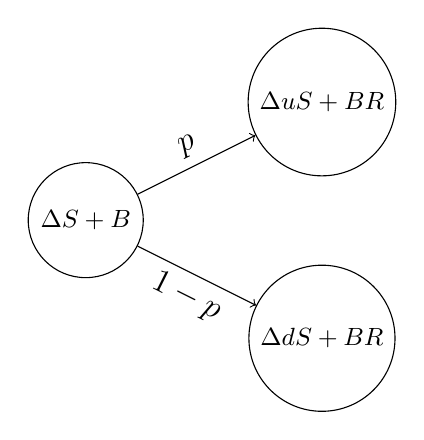
\begin{tikzpicture}
    \node[malnode] (init) at (0,0) {$\Delta S+B$};
    \node[malnode] (up) at (3, 1.5) {$\Delta uS+BR$};
    \node[malnode] (down) at (3, -1.5) {$\Delta dS+BR$};
    \draw[->] (init) -- (up) node[prob, above] {$p$};
    \draw[->] (init) -- (down) node[prob, below] {$1-p$};

\end{tikzpicture}
\end{center}

Ainsi, comme le portefeuille réplique $C$, on obtient :
\begin{align*}
    \left\{ \begin{array}{cl}
    \Delta uS + BR&=C_u \\
    \Delta dS + BR&=C_d \\
    \end{array} \right. \implies \Delta S(u-d) = C_u-C_d \implies \Delta=\frac{C_u-C_d}{S(u-d)}
\end{align*}
De plus,
\begin{align*}
    \left\{ \begin{array}{cl}
    &\Delta uS + BR=C_u \\
    &\Delta dS + BR=C_d \\
    \end{array} \right. \iff  
    \left\{ \begin{array}{cl}
    -\Delta udS - dBR&=-dC_u \\
    \Delta udS + uBR&=uC_d \\
    \end{array} \right. \\
    \implies RB(u-d)=uC_d-dC_u
    \implies B=\frac{uC_d-dC_u}{R(u-d)}
\end{align*}
En remplaçant,
\begin{align*}
    C = \Delta S+B &= \frac{C_u-C_d}{S(u-d)}S+\frac{uC_d-dC_u}{R(u-d)} =\frac{R(C_u-C_d)+uC_d-dC_u}{R(u-d)} \\ 
    &=\frac{1}{R}\bigg(\frac{R-d}{u-d}C_u+\frac{u-R}{u-d}C_d\bigg) \\
    &=\frac{1}{R}(pC_u+(1-p)C_d), \text{ avec } p=\frac{R-d}{u-d} \text{ et } 1-p = \frac{u-R}{u-d} \\
\end{align*}
\remarque On a bien $1 = p + (1 - p) = \dfrac{R-d+u-R}{u-d} = 1$.\\ On a aussi nécessairement $d<R<u$.
En effet, 
\begin{description}
    \item[Si $R \leq d < u$ :] On emprunte au taux sans risque 
    \begin{itemize}
        \item En cas de baisse : $dS_0-RS_0=S_0(d-R) \geq 0$
        \item En cas de hausse : $uS_0-RS_0 = S_0(u-R) \geq 0$
    \end{itemize}
    \item[Si $d < u \leq R$ :] On vend à découvert
    \begin{itemize}
        \item En cas de hausse : $RS_0-uS_0 = S_0(R-u) \geq 0$
        \item En cas de baisse : $RS_0-dS_0 = S_0(R-d) \geq 0$
    \end{itemize}
\end{description}
Dans les quatre cas, on obtient un arbitrage ce qui contredit l'A.O.A. Ainsi, le rendement sans risque est strictement compris entre les meilleurs et pires rendements risqués. \\
On peut réécrire la formule en utilisant la probabilité risque-neutre. \\

\begin{definitionbox}[frametitle = {Formule d'évaluation risque-neutre}]
    Soient $u$ et $d$ les facteurs d'évolution avec $d < R < u$ où $R$ est le facteur sans risque, et $C_u, C_d$ les flux futurs de l'option : 
    \begin{align*}
         C_0&=\dfrac{1}{R}(pC_u+(1-p)C_d), \text{ avec } p=\dfrac{R-d}{u-d} \text{ et } 1-p = \dfrac{u-R}{u-d} \\
         &=\frac{\mathbb{E}^{\mathbb{Q}}(C_1)}{R}, \text{ avec } \mathbb{Q} \text{ la mesure de probabilité risque-neutre} \\
    \end{align*}
\end{definitionbox}

\subsection{Raisonnement Rétrograde}
On peut maintenant appliquer le principe dit de \textbf{Raisonnement Rétrograde} ou de \textbf{Backward Induction}. Ce principe consiste à partir de la fin de l'arbre puis remonter sur le noeud précédent pour calculer sa valeur égale à l'espérance des noeuds suivants et répétant itérativement jusqu'à l'origine. Du fait de la nature non linéaire des formules d'évaluations des calls et puts (max), on ne peut savoir la valeur des noeuds terminaux qu'à la fin de la construction de l'arbre. On a alors besoin de construire l'arbre une première fois avant de le remonter. Ce principe est également très utile pour gérer les \textbf{options américaines} ainsi que pour le \textbf{delta hedging}. \\
~\\
On considère le morceaux d'arbre suivant :
\tikzset{
   malnode/.style={draw=black, fill=white, minimum width=3.5em, circle, font=\small},
   prob/.style={midway, sloped, font=\large},
   malarrow/.style={->, >=stealth, shorten >=2pt, shorten <=2pt}
}
\begin{center}
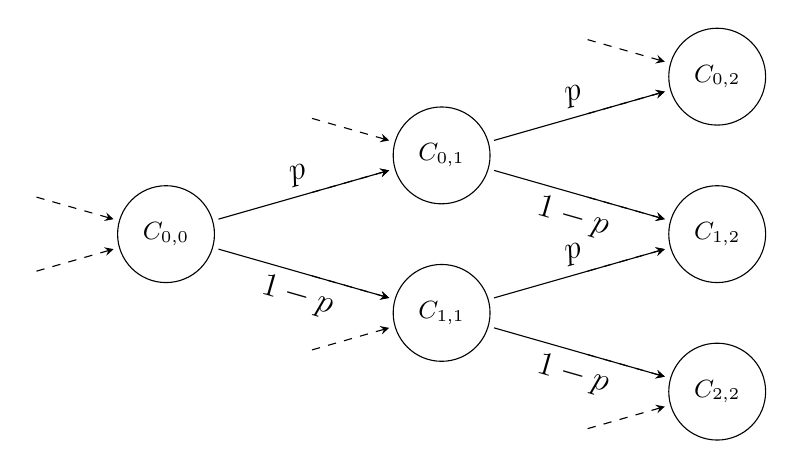
\begin{tikzpicture}
\foreach \x in {0,...,2} { 
    \foreach \y in {0,...,\x} { 
        \pgfmathsetmacro{\movey}{\y - \x/2}
        \def\nodetext{?}
        \ifnum\x=0
            \def\nodetext{$C_{0,0}$}
        \fi
        \ifnum\x=1
            \ifnum\y=1 \def\nodetext{$C_{0,1}$} \fi
            \ifnum\y=0 \def\nodetext{$C_{1,1}$} \fi
        \fi
        \ifnum\x=2
            \ifnum\y=2 \def\nodetext{$C_{0,2}$} \fi
            \ifnum\y=1 \def\nodetext{$C_{1,2}$} \fi
            \ifnum\y=0 \def\nodetext{$C_{2,2}$} \fi
        \fi
        \node[malnode] (\x-\y) at (3.5*\x, 2.0*\movey) {\nodetext};
        \draw[malarrow, dashed, <-] (\x-\y) -- ++(-\ratiox*0.5, \ratioy*0.25);
        \draw[malarrow, dashed, <-] (\x-\y) -- ++(-\ratiox*0.5, -\ratioy*0.25);
        \ifnum\x>0
            \pgfmathtruncatemacro{\prevx}{\x-1}
            \ifnum\y>0
                \pgfmathtruncatemacro{\prevyup}{\y-1}
                \draw[malarrow] (\prevx-\prevyup) -- (\x-\y) node[prob, above] {$p$};
            \fi
            \ifnum\y<\x
                \draw[malarrow] (\prevx-\y) -- (\x-\y) node[prob, below] {$1-p$};
            \fi
        \fi
    }
}
\end{tikzpicture}
\end{center}
En utilisant le raisonnement rétrograde, on peut exprimer la valeur du noeud $C_{0,1}$ à partir de celles de $C_{0,2}$ et $C_{1,2}$. On obtient alors : 
$$C_{0,1} = \frac{1}{R}(pC_{0,2}+(1-p)C_{1,2})$$
Ainsi, on peut remonter l'arbre en partant des feuilles pour évaluer l'ensemble des noeuds précédents: 
$$C_{i,t}=\frac{1}{R}(pC_{i,t+i}+(1-p)C_{i,t})$$
avec $i$ la position du noeud parmi les noeuds de profondeur $t$.
Les valeurs des feuilles sont données par la formule du call (resp. put) si on modélise un call (resp. put). Ici, on aura : $C_{i} = max(S-K,0)$ avec $S$ le prix du sous-jacent et $K$ le strike. 
\vspace{0.02\textheight}\\
Appliquons le modèle binomial sur une option dans l'exemple suivant: \\
\vspace{0.01\textheight}
\underline{Données} : 
\begin{itemize}
    \item Prix actuel : $S_0$
    \item Prix d'exercice : $K = 100\$$
    \item Facteur de hausse : $u = 1,1$
    \item Facteur de baisse : $d = 0,9$
    \item Taux sans risque : $r = 0.05$ donc $R=1.05$
    \item Nombre de périodes : $N=2$
\end{itemize}
\vspace{0.01\textheight}
\underline{Phase de descente :} \\
On calcule les trajectoires possibles
\begin{description}
    \item[Temps t=1:] ~\
        \begin{itemize}
            \item $S_u = 100 \times 1,1 = 110$
            \item $S_d = 100 \times 0,9 = 90$
        \end{itemize}
    \item[Temps t=2:] ~\
        \begin{itemize}
            \item $S_{uu} = 110 \times 1,1 = 121$
            \item $S_{ud} = 110 \times 0,9 = 99$
            \item $S_{dd} = 90 \times 0,9 = 81$
        \end{itemize}
\end{description}
\vspace{0.01\textheight}
\underline{Calcul des probabilités risque-neutres :}
$$p = \frac{R - d}{u - d} = \frac{1,05 - 0,9}{1,1 - 0,9} = \frac{0,15}{0,20} = 0,75$$
\vspace{0.01\textheight}
\underline{Calcul des valeurs des feuilles :} \\
On calcule le payoff du Call : 
\begin{itemize}
    \item $C_{uu} = \max(121 - 100, 0) = 21$
    \item $C_{ud} = \max(99 - 100, 0) = 0$
    \item $C_{dd} = \max(81 - 100, 0) = 0$
\end{itemize}
\vspace{0.01\textheight}
\underline{Phase de remontée :} \\
\begin{description}
    \item[Temps t = 1:] 
        \begin{align*}
            C_u &= \frac{1}{1,05} (0,75 \cdot 21 + 0,25 \cdot 0) = \frac{15,75}{1,05} = 15\\
            C_d &= \frac{1}{1,05} (0,75 \cdot 0 + 0,25 \cdot 0) = 0
        \end{align*}
    \item[Temps t = 0:]
        \begin{align*}
            C_0 = \frac{1}{1,05}(0.75 \cdot15+0.25\cdot0) = \frac{11.25}{1.05} \approx 10.71
        \end{align*}
\end{description}
Pour cette option, le prix juste à exiger est de $10.71 \$$
\subsection{Options Américaines}

